\documentclass{article}

\usepackage{tikz}
\usetikzlibrary{
    arrows.meta, % for the special arrow tip
    backgrounds, % for the two rectangular areas that are behind the two main parts
    decorations.pathmorphing, % for the “snaking line” in the middle
    fit, % to easily compute the sizes of these rectangles
    petri, % defines a place style
    positioning % for placing nodes relative to other nodes
}

% epigraph for quote at start of section
\usepackage{epigraph}
\setlength\epigraphwidth{8cm}
\setlength\epigraphrule{0pt}
\renewcommand{\epigraphsize}{\small\itshape}

% for hyperlinks and URL links
\usepackage{hyperref}

\title{\LaTeX{} Experiments\\ Part III-B: PGF/TikZ - A Petri net example}

\author{AeAeA}

\begin{document}

\maketitle

\newpage
%==============================================================================
\section{What is a Petri net?}

\epigraph
{There is a theory which states that if ever anyone discovers exactly what the 
Universe is for and why it is here, it will instantly disappear and be replaced 
by something even more bizarre and inexplicable. \\
\hfill \break
There is another theory which states that this has already happened.}
{--- \textup{Douglas Adams},\\ The Restaurant at the End of the Universe}

\begin{itemize}

    \item Quick intro:\\ 
          \url{https://en.wikipedia.org/wiki/Petri_net}
    
    \item A good basic explanation of what is a 
          \href{https://www.techfak.uni-bielefeld.de/~mchen/BioPNML/Intro/pnfaq.html}
          {Petri net}, with a 
          \href{https://www.techfak.uni-bielefeld.de/~mchen/BioPNML/Intro/MRPN.html}
          {well-illustrated example}.

    \item Petri nets and algebraic specifications 
          \href{https://www.sciencedirect.com/science/article/pii/030439759190203E?via%3Dihub}
          {paper} (1991).

\end{itemize}

\newpage
%==============================================================================
\section{The Complete Code}

\epigraph
{The story so far: \\
\hfill \break
In the beginning the Universe was created.\\
\hfill \break
This has made a lot of people very angry and been widely regarded as a bad move.}
{--- \textup{Douglas Adams},\\ The Restaurant at the End of the Universe}

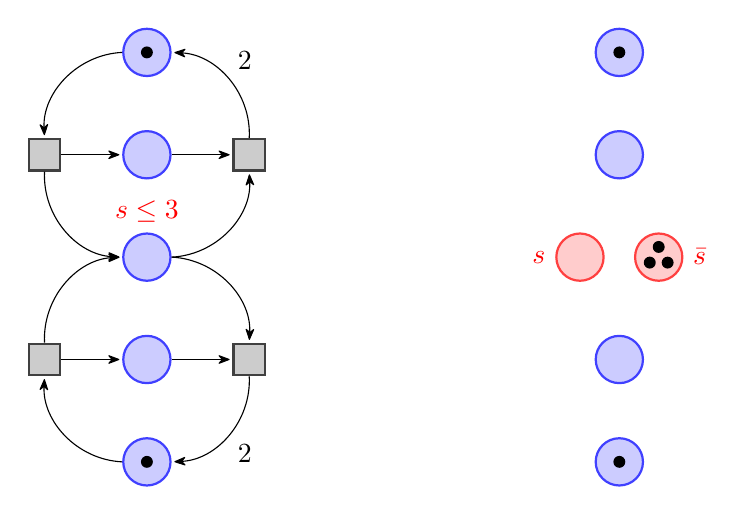
\begin{tikzpicture}[
    node distance=1.3cm,on grid,>={Stealth[round]},bend angle=45,auto,
    every place/.style      = {minimum size=6mm,thick,draw=blue!75,fill=blue!20}, 
    every transition/.style = {thick,draw=black!75,fill=black!20},
    red place/.style        = {place,draw=red!75,fill=red!20},
    every label/.style      = {red}
]

% Petri net with capacity place (left)

    \node [place,tokens=1] (w1)                                    {};
    \node [place]          (c1) [below=of w1]                      {}; 
    \node [place]          (s)  [below=of c1,label=above:$s\le 3$] {}; 
    \node [place]          (c2) [below=of s]                       {};
    \node [place,tokens=1] (w2) [below=of c2]                      {};

    \node [transition] (e1) [left=of c1]  {}
        edge [pre,bend left]                  (w1) 
        edge [post,bend right]                (s) 
        edge [post]                           (c1);
    \node [transition] (e2) [left=of c2]  {}
        edge [pre,bend right]                 (w2) 
        edge [post,bend left]                 (s) 
        edge [post]                           (c2);
    \node [transition] (l1) [right=of c1] {}
        edge [pre]                            (c1) 
        edge [pre,bend left]                  (s) 
        edge [post,bend right] node[swap] {2} (w1);
    \node [transition] (l2) [right=of c2] {}
        edge [pre]                            (c2) 
        edge [pre,bend right]                 (s) 
        edge [post,bend left]  node {2}       (w2);

% Equivalent Petri net with place complementation (right)

\begin{scope}[xshift=6cm]

    \node [place,tokens=1]     (w1')                                                   {};
    \node [place]              (c1') [below=of w1']                                    {};
    \node [red place]          (s1') [below=of c1',xshift=-5mm] [label=left:$s$]       {};
    \node [red place,tokens=3] (s2') [below=of c1',xshift=5mm]  [label=right:$\bar s$] {};
    \node [place]              (c2') [below=of s1',xshift=5mm]                         {};
    \node [place,tokens=1]     (w2') [below=of c2']                                    {};
    

\end{scope}

\end{tikzpicture}


\end{document}